\chapter{Implementierung des Copyright-Scanners}\label{ch:copyright-scanner}

Das vorliegende Kapitel widmet sich der konkreten Implementierung des Copyright-Scanners.
Die Konzeption des Prototyps leitet sich direkt aus den Erkenntnissen der vorangegangenen Kapitel ab, insbesondere aus den Ergebnissen des Benchmarks und der darauf aufbauenden Optimierungen durch Prompt-Engineering und Fine-Tuning.
Während die in Kapitel 7 beschriebene Benchmark-Implementierung primär der Evaluation und dem Vergleich verschiedener Modelle diente und dafür umfassende Mechanismen zur Metrikerhebung und Validierung umfasste, konzentriert sich die hier vorgestellte Umsetzung auf die funktionale Kernkomponente und ihre Integration in einen übergeordneten Verarbeitungsprozess.
Zunächst wird die grundlegende Konzeption des Systems erläutert, gefolgt von einer Beschreibung der Schnittstellen und der potenziellen Integration in bestehende Systeme.

% ======================================================================================================================

\section{Konzeption}

Die Abbildung~\ref{fig:copyright-scanner} veranschaulicht den konzeptionellen Aufbau und den Datenfluss des Copyright-Scanners.
Sie zeigt die Interaktion zwischen dem Java-Backend, dem in einem Docker-Container gekapselten \gls{llm} und den angebundenen Datenquellen sowie nachgelagerten Prozessen.
Der Ablauf der Verarbeitung gliedert sich in sechs wesentliche Schritte.

\begin{figure}[ht]
    \centering
    \makebox[\textwidth]{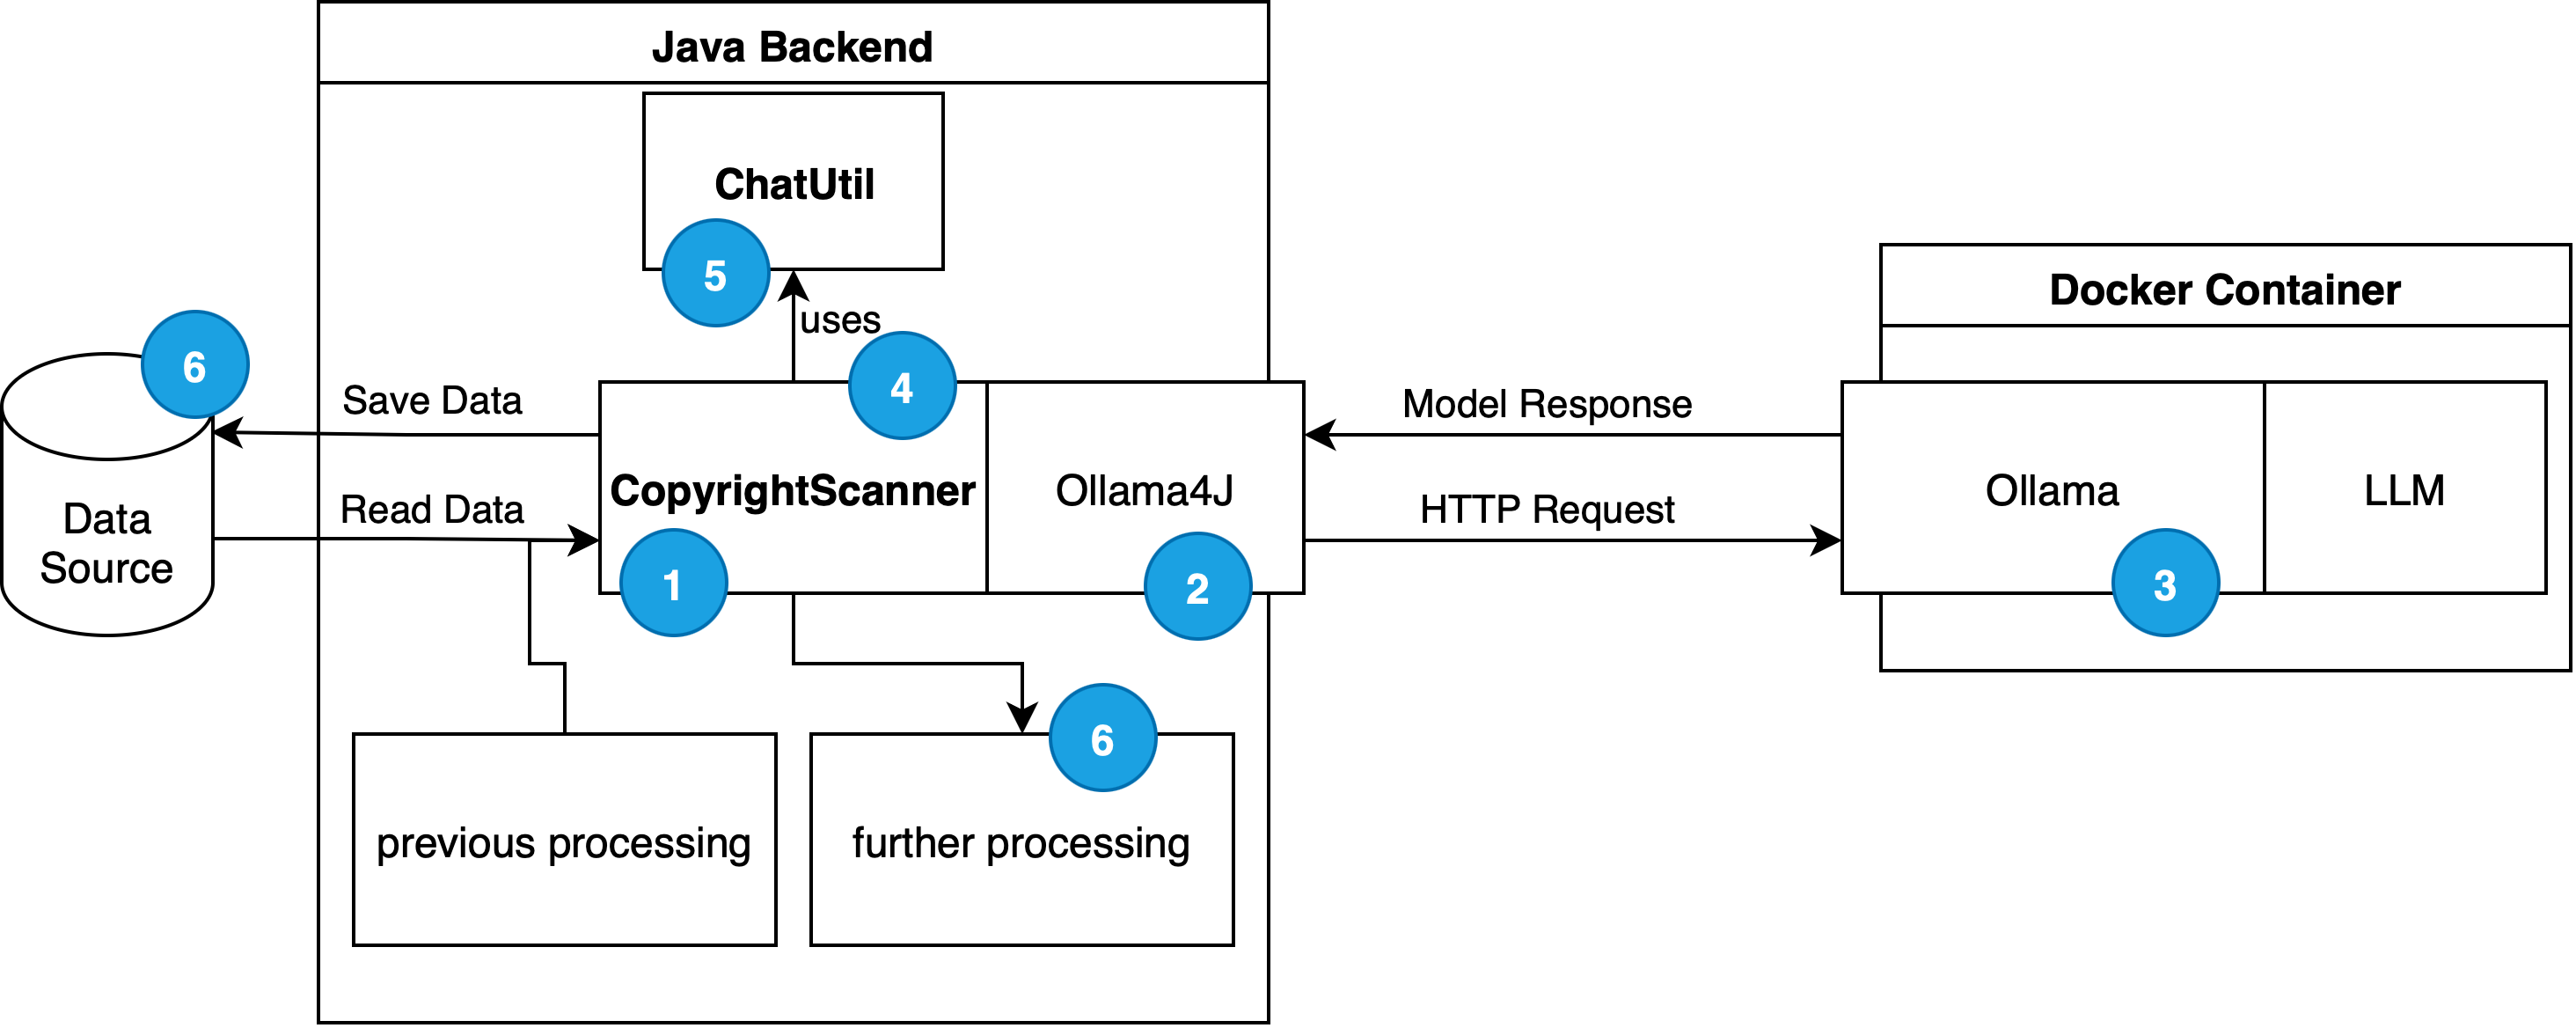
\includegraphics[width=1.3\textwidth]{copyright-scanner/copyright-scanner-sketch.png}}
    \caption{Schematische Darstellung der Architektur und des Datenflusses des Copyright-Scanners. Das Diagramm verdeutlicht die modulare Architektur, die eine klare Trennung zwischen der Verarbeitungslogik im Java-Backend und dem in einem Docker-Container gekapselten Sprachmodell sicherstellt.}
    \label{fig:copyright-scanner}
\end{figure}

Der Prozess beginnt im CopyrightScanner (1), der Eingabedateien von einem vorgelagerten Prozess oder direkt aus einer Datenquelle erhält.
Diese Dateien werden zunächst anhand einer Wortliste gefiltert, um sie auf Copyright-relevante Inhalte zu reduzieren.
Danach wird der gefilterte Inhalt mit einem Extraktionsprompt kombiniert und über die Ollama4J-Schnittstelle (2) als Anfrage an den Ollama-Dienst gesendet.
Der Ollama-Dienst (3), der in einem Docker-Container gekapselt ist, nimmt diese Anfrage entgegen.
Er verwaltet das zugrundeliegende LLM, führt die Inferenz aus und sendet die generierte Antwort zurück an das Java-Backend.
Im CopyrightScanner (4) wird die empfangene Antwort validiert, indem versucht wird, sie als valides JSON zu parsen.
Falls dieser Schritt fehlschlägt, etwa weil die Antwort zusätzliche textuelle Artefakte enthält, wird die ChatUtil-Klasse (5) verwendet, um die Ausgabe zu bereinigen und ein gültiges JSON-Objekt zu extrahieren.
Die erfolgreich extrahierten und validierten Informationen werden abschließend (6) entweder in der Datenquelle gespeichert oder an nachfolgende Verarbeitungsschritte übergeben.

% ======================================================================================================================

\section{Beschreiben der Schnittstellen und Integration in bestehende Systeme}

Die Integration des entwickelten Copyright-Scanners in bestehende Prozessketten stellt eine zentrale Anforderung dar, die maßgeblich durch die Gestaltung seiner Schnittstellen bestimmt wird.
Die primäre Schnittstelle des Systems ist für die Entgegennahme von Eingabedateien und die Bereitstellung der extrahierten Ergebnisse konzipiert.
Intern kommuniziert der Scanner, wie in Abbildung~\ref{fig:copyright-scanner} dargestellt, über die Ollama4J-Bibliothek, die eine REST-API-Schnittstelle zum lokal ausgeführten Ollama-Dienst kapselt.
Diese Architektur ermöglicht eine flexible Bereitstellung, bei der das Sprachmodell unabhängig von der verarbeitenden Anwendung auf derselben oder einer anderen Maschine im Netzwerk betrieben werden kann, was dem im Anwendungsszenario geforderten On-Premise-Betrieb entgegenkommt.

Ein entscheidender Vorteil für die Integration in bestehende Systeme der metaeffekt ist die bewusste Entscheidung, das Ausgabeformat des Scanners an das JSON-Schema des ScanCode-Toolkits anzugleichen.
Bestehende nachgelagerte Prozesse, die bereits auf die Verarbeitung der ScanCode-Ergebnisse ausgelegt sind, können die vom LLM-basierten Scanner generierten Daten somit ohne wesentliche Anpassungen weiterverarbeiten.
Diese Kompatibilität vereinfacht die Einführung der neuen Lösung erheblich, da sie als direkter Ersatz oder als ergänzende Komponente in der bestehenden Werkzeugkette fungieren kann.

Allerdings stellt die Ausführung des Systems höhere Anforderungen an die Hardware als traditionelle, regelbasierte Werkzeuge.
Die Inferenz eines \glspl{llm} ist rechen- und speicherintensiv.
Wie die Untersuchungen in Kapitel~\ref{ch:benchmark} gezeigt haben, ist für eine performante lokale Ausführung leistungsfähige Hardware erforderlich, beispielsweise ein System mit ausreichend Arbeitsspeicher und einer leistungsstarken GPU wie der im Benchmark verwendete Mac Mini.
Unternehmen, die eine Integration in Erwägung ziehen, müssen diesen Aspekt berücksichtigen, da die Notwendigkeit spezieller Hardware eine Hürde für die Implementierung darstellen kann.
